%=================== HEADER =====================%
% Basic Document Formatting
\documentclass[12pt,a4paper]{article}
\usepackage[T1]{fontenc}
\usepackage[utf8]{inputenc}
\usepackage[left=1in, right=1in, top=0.9in]{geometry}

% Other Preamble
\usepackage{setspace}

\usepackage{fancyhdr}
\setlength{\parindent}{0in}

% Page Formatting
\pagenumbering{arabic} %\pagenumbering{gobble}
\onehalfspacing %doublespacing
\pagestyle{fancy}
\usepackage{pdfpages}

% Heading Formatting
\headheight 32pt

% Link Formatting
\usepackage{hyperref}
\hypersetup{
	colorlinks,
	allcolors=black
	%citecolor=black,
	%filecolor=black,
	%linkcolor=black,
	%urlcolor=black
}

\usepackage{mdframed}

% Code Formatting
\usepackage{listings}
\lstset{
	basicstyle=\footnotesize,
	numbers=left,
	stepnumber=1,
	showstringspaces=false,
	tabsize=1,
	breaklines=true,
	breakatwhitespace=false
}

% Figures & Drawings
\usepackage{graphicx, caption}
\usepackage{animate}
\usepackage{tikz}
\usepackage{float}
\usepackage{pict2e}

% Physics
\usepackage{physics}

% Mathematics
\usepackage{amsmath}
\usepackage{amssymb}
\usepackage{amsthm}
\usepackage{mathtools}
\usepackage{upgreek} % More Greek letters

% I don't really know what this is but I don't want to break shit
\usepackage{aliascnt}
\newaliascnt{eqfloat}{equation}
\newfloat{eqfloat}{h}{eqflts}
\floatname{eqfloat}{Equation}
\newcommand*{\ORGeqfloat}{}
\let\ORGeqfloat\eqfloat
\def\eqfloat{%
	\let\ORIGINALcaption\caption
	\def\caption{%
		\addtocounter{equation}{-1}%
		\ORIGINALcaption
	}%
	\ORGeqfloat
}


%}

% Bibliography (Citations) Formatting

%\usepackage{cite}
\usepackage{caption}
\usepackage[backend=bibtex,style=apa]{biblatex} %works really really well, but no MLA format
%\usepackage[backend=biber,style=mla]{biblatex} %Doesn't print all sources for some reason
% Custom Symbols 
%{
\newcommand\halmos{\rule{.36em}{2ex}} % Custom QED Symbol
\def\contradict{\tikz[baseline, x=0.22em, y=0.22em, line width=0.032em]\draw (0,2.83)--(2.83,0) (0.71,3.54)--(3.54,0.71) (0,0.71)--(2.83,3.54) (0.71,0)--(3.54,2.83);}
\renewcommand{\qedsymbol}{\halmos}
\renewenvironment{proof}{{\bfseries \textit{Proof} \\}}{\qedsymbol}

\makeatletter
\newcommand{\crossout}[1]{% Crosses out symbol
	\begingroup
	\settowidth{\dimen@}{#1}%
	\setlength{\unitlength}{0.05\dimen@}%
	\settoheight{\dimen@}{#1}%
	\count@=\dimen@
	\divide\count@ by \unitlength
	\begin{picture}(0,0)
		\put(0,0){\line(20,\count@){20}}
		\put(0,\count@){\line(20,-\count@){20}}
	\end{picture}%
	#1%
	\endgroup
}
%}

% Mathematics (General)
\newtheorem{theorem}{Theorem}[section]
\newtheorem{corollary}{Corollary}[theorem]
\newtheorem{lemma}[theorem]{Lemma}

\newcommand{\lemref}[1]{\textit{Lemma \ref{#1}}}
\newcommand{\thmref}[1]{\textbf{Theorem \ref{#1}}}
\newcommand{\colref}[1]{\textit{Corollary \ref{#1}}}

% Physics (Quantum Mechanics)
%\newcommand{\norm}[#1]{\lVert {#1} \rVert}
%\newcommand{\ket}[1]{\vert{#1}\rangle}
%\newcommand{\bra}[1]{\langle{#1}\vert}
%\newcommand{\braket}[2]{\langle {#1} \vert {#2} \rangle}
\newcommand{\expectation}[1]{\langle{#1}\rangle}

% Physics (Electrodynamics)
\newcommand{\del}{\overline{\nabla}}
\usetikzlibrary{arrows}
%Script r (scalar)
\newcommand{\rc}{%
\resizebox{!}{1.25ex}{%
    \begin{tikzpicture}[>=round cap]
        \clip (0.09em,-0.05ex) rectangle (0.61em,0.81ex);
        \draw [line width=.11ex, <->, rounded corners=0.13ex] (0.1em,0.1ex) .. controls (0.24em,0.4ex) .. (0.35em,0.8ex) .. controls (0.29em,0.725ex) .. (0.25em,0.6ex) .. controls (0.7em,0.8ex) and (0.08em,-0.4ex) .. (0.55em,0.25ex);
    \end{tikzpicture}%
}%
}

%Script r (vector)
\newcommand{\brc}{%
\resizebox{!}{1.3ex}{%
    
\begin{tikzpicture}[>=round cap]
        \clip (0.085em,-0.1ex) rectangle (0.61em,0.875ex);
        \draw [line width=.2ex, <->, rounded corners=0.13ex] (0.1em,0.1ex) .. controls (0.24em,0.4ex) .. (0.35em,0.8ex) .. controls (0.29em,0.725ex) .. (0.25em,0.6ex) .. controls (0.7em,0.8ex) and (0.08em,-0.4ex) .. (0.55em,0.25ex);
    \end{tikzpicture}%
}%
}

%Script r with a hat (unit vector)
\newcommand{\hrc}{\hat{\brc}}


% Document (General)
\newcommand{\figref}[1]{Fig. \ref{#1}}
\newcommand{\source}[1]{\caption*{Source: {#1}} }
\newcommand{\sourceref}[1]{\caption*{Source: {\fullcite{#1}}}}
\tikzset{>=latex} % for LaTeX arrow head
\colorlet{myred}{red!85!black}
\colorlet{mydarkred}{red!55!black}
\colorlet{mylightred}{red!85!black!12}
\colorlet{myfieldred}{mydarkred!5} % for S' background
\colorlet{myredhighlight}{myred!20} % highlights simultaneity in ladder paradox
\colorlet{myblue}{blue!80!black}
\colorlet{mydarkblue}{blue!50!black}
\colorlet{mylightblue}{blue!50!black!30}
\colorlet{mylightblue2}{myblue!10}
\colorlet{mygreen}{green!80!black}
\colorlet{mypurple}{blue!40!red!80!black}
\colorlet{mydarkgreen}{green!50!black}
\colorlet{mydarkpurple}{blue!40!red!50!black}
\colorlet{myorange}{orange!40!yellow!95!black}
\colorlet{mydarkorange}{orange!40!yellow!85!black}
\colorlet{mybrown}{brown!20!orange!90!black}
\colorlet{mydarkbrown}{brown!20!orange!55!black}
\colorlet{mypurplehighlight}{mydarkpurple!20} % highlights simultaneity in ladder paradox
\tikzstyle{world line}=[myblue!40,line width=0.3]
\tikzstyle{world line t}=[mypurple!50!myblue!40,line width=0.3]
\tikzstyle{world line'}=[mydarkred!40,line width=0.3]
\tikzstyle{mysmallarr}=[-{Latex[length=3,width=2]},thin]
\tikzstyle{mydashed}=[dash pattern=on 3 off 3]
\tikzstyle{rod}=[mydarkbrown,draw=mydarkbrown,double=mybrown,double distance=2pt,
                 line width=0.2,line cap=round,shorten >=1pt,shorten <=1pt]
%\tikzstyle{rod'}=[rod,draw=mydarkbrown!80!red!85,double=mybrown!80!red!85]
\tikzstyle{vector}=[->,line width=1,line cap=round]
\tikzstyle{vector'}=[vector,shorten >=1.2]
\tikzstyle{particle}=[mygreen,line width=0.9]
\tikzstyle{photon}=[-{Latex[length=5,width=4]},myorange,line width=0.8,decorate,
                    decoration={snake,amplitude=1.0,segment length=5,post length=5}]

\def\tick#1#2{\draw[thick] (#1) ++ (#2:0.06) --++ (#2-180:0.12)}
\def\tickp#1#2{\draw[thick,mydarkred] (#1) ++ (#2:0.06) --++ (#2-180:0.12)}
\def\Nsamples{100} % number samples in plot
\usepackage{mathrsfs}
\bibliography{references.bib}

%============ Document Information ==============%
\newcommand\course{ESS205} %[COURSE INFORMATION!!!]
\newcommand\psetnum{Geothermal Energy in Canada}  %[PROBLEM SET NUMBER!!!]
\newcommand\yourname{Aditya Rao 1008307761 \\ Andrew Lehmann 1008751405}  %[NAME AND STUDENT NUMBER!!!]
\newcommand{\subject}{\large{\course}}
%================ END OF HEADER =================%

% LaTeX Template by Aditya Rao

\begin{document}
    \title{\psetnum \\ \large{\course}}
	\author{\yourname}
	\date{January 30, 2024}
	\maketitle

	%\pagenumbering{roman}

	%\tableofcontents
	
	%\newpage
	%So the heading doesn't show up on table of contents page
	%\lhead{\yourname\ \vspace{0.1cm} \\ \course}
	\lhead{\yourname\ \vspace{0.1cm}}
    \chead{\textbf{\subject} \\ \psetnum}
    \rhead{\leftmark}

    \section[Topic]{Geothermal Energy in Canada}
        Our topic will focus on current methods of geothermal energy production in Canada with a focus on the current efforts in Ontario.
        
        \textbf{Method: Paper}

        
    \section{Three Key Papers}
        \subsection{Paper 1: \textit{Geothermal Energy in Canada, Jessop et al.}}
            \textbf{\fullcite{geothermal_energy_in_canada}}
            
            \vspace{0.5cm}
            
            This source provides a good general overview of the state of Geothermal energy in Canada. It focuses on two major regions: the Meager Mountain volcanic complex in British Columbia and the Western Platform in British Columbia. It is observed that the potential thermal energy of the water temperature of the Western Platform is ``very large'' with only ``1\% of the resource base'' being almost $10\times$ the estimated thermal equivalent of Canada's oil reserves. The paper further goes into logistics difficulties in creating geothermal plants in Eastern Canada (i.e. Ontario).

        \subsection{Paper 2: \textit{Geothermal Energy Resource Potential of Canada, Grasby et al.}}
            \textbf{\fullcite{govt_canada_2022}}

            \vspace{0.5cm}
            This source is a geological survey that provides an overview of Canada's potential to incorporate geothermal energy into its electrical grid and transition away from fuels that use hydrocarbons. The extensive survey delves also delves into the geological challenges, and regulatory issues that may arise. 


        \subsection{Paper 3:Supercritical Thermodynamics of the Rock/Fluid Geothermal System.}
            \textbf{\fullcite{suárez_2021}}
            
            \vspace{0.5cm}
            This paper is relevant to geothermal energy in Canada, as it defines a concise mathematical description of the behaviour of water in the supercritical region. The supercritical state of fluid of a given substance at a temperature and pressure above its critical point may overcome limitations from mass transfer in fluids, significantly increasing efficiency in geothermal systems. Many power generation systems use water as their primary working fluid, and increasing the temperature of the water will increase its power output and efficiency, which implies having a paper that details the behaviour of water in this state is applicable. 

    \section[Diagram]{Quantitative Diagram or Map}
        \begin{figure}[H]
            \captionsetup{{width=0.7\linewidth}}
            \centering
            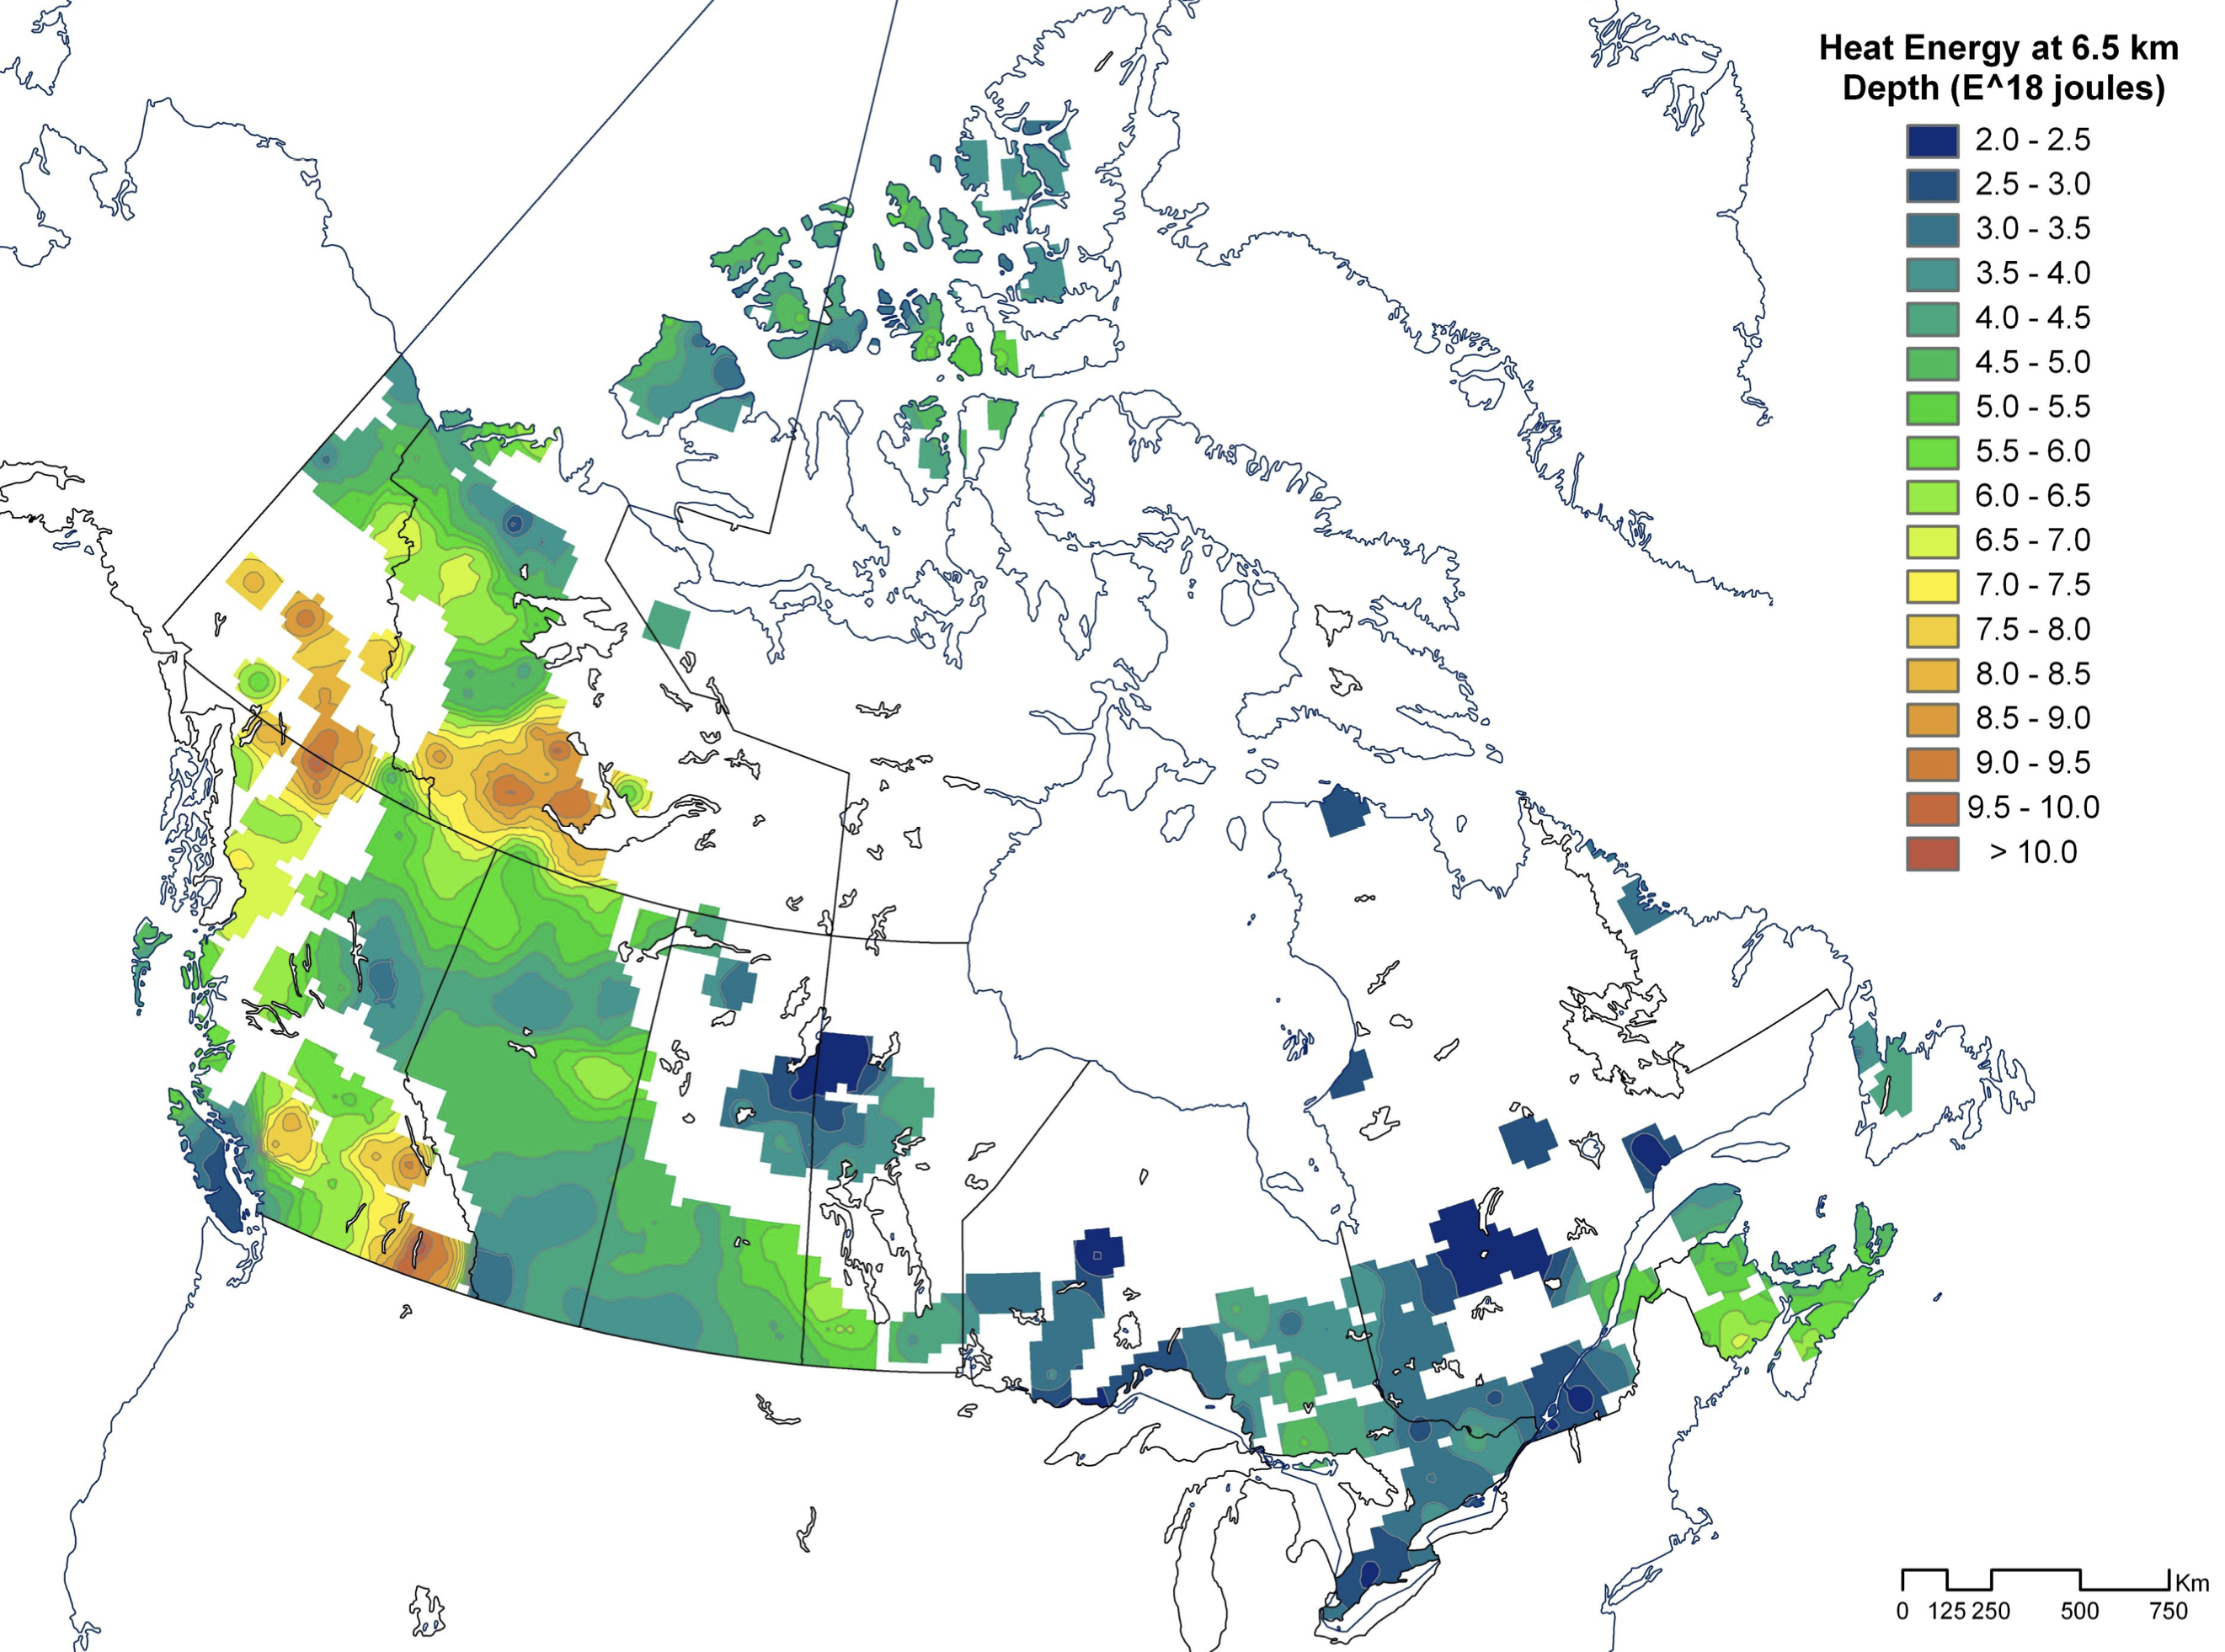
\includegraphics[width=0.7\textwidth]{figures/diagram.png}
            \caption{Quantitative Diagram}
            \textbf{\sourceref{govt_canada_2022}}
        \end{figure}

        %\subsection{Diagram Reference}
        %    The diagram was found at\autocite{diagram_ref}
        
        \subsection{Visual's usefulness to topic}
            This provides a general basis for describing Canada's heat capacity at a certain depth. It will be useful in discussing the real-world applications of our analysis of the thermodynamic effects of geothermal energy in Canada.
		
    %\newpage
    \section{References}
        \nocite{*}
        \printbibliography[heading=none]

\end{document}